\input{mlClassDefs.tex}

\oddsidemargin 0in
\evensidemargin 0in
\textwidth 6.5in
\topmargin -0.5in
\textheight 9.0in

\begin{document}

\solution{Gen Nishida}{\today}{2}{Fall 2014}
% Fill in the above, for example, as follows:
% \solution{John Smith}{\today}{1}{Fall 2014}

\pagestyle{myheadings}  % Leave this command alone

\section{Questions}

\begin{enumerate}
\item 
(1) Boolean function

By using conjunctions for every combination of three variables, we can test if at least three variables are active. Therefore, the Boolean function for this is as follows:
\begin{eqnarray*}
f=(x_1 \wedge x_2 \wedge x_3) \vee (x_1 \wedge x_2 \wedge x_4) \vee (x_1 \wedge x_2 \wedge x_5) \vee (x_1 \wedge x_3 \wedge x_4) \vee (x_1 \wedge x_3 \wedge x_5) \\
\vee (x_1 \wedge x_4 \wedge x_5) \vee (x_2 \wedge x_3 \wedge x_4) \vee (x_2 \wedge x_3 \wedge x_5) \vee (x_2 \wedge x_4 \wedge x_5) \vee (x_3 \wedge x_4 \wedge x_5)
\end{eqnarray*}

(2) Linear function

Linear function that can achieve the same classification just needs to checke if the sum is more than two.
\[
f = \begin{cases}
1 & (x_1 + x_2 + x_3 + x_4 + x_5 \geq 3) \\
0 & Otherwise
\end{cases}
\]


\item What is the size of $CON_B$?

For every variable, there are two cases, used in the conjunctions or not used. Thus, the size of $CON_B$ is $2^n$. 

\item What is the size of $CON_L$?

For every pair of $f_b^{(i)}$ and $f_b^{(j)}$ $(i \neq j)$ in $CON_B$, $\exists x, f_b^{(i)} \neq f_b^{(j)}$. Thus, ths size of $CON_L$ has to be larger than the size of $CON_B$ to make it consistent with $CON_B$. However, 

\item Mistake bound

Mistake bound is the maximum possible number of mistakes made by the online learning algorithms, which is also used to evaluate the performance of the convergence of the algorithms. 

\item mistake bound algorithm

1) initialize the hypothesis: $f = x_1 \wedge \neg x_1 \wedge x_2 \wedge \neg x_2 \wedge \cdots \wedge x_n \wedge \neg x_n$ \\
2) if no mistake do nothing \\
3) else \\
4)    for all in-active variables, remove $x_i$ from the conjunctions \\ 

The example of the learning process is shown in Figure \ref{fig:learning_process}. For instance, when the first mistake is made for an example $x=(1, 0, 0)$, the variables $\neg x_1$, $ x_2$, and $x_3$ are in-active, and these variables are removed from the conjunctions, which results in the updated hypothesis $f = x_1 \wedge \neg x_2 \wedge \neg x_3$. 

For every mistake, we remove at least one unnecessary variable from the conjunctions. Since we have at least one variable in the conjunctions, the total number of mistakes is at most $2n-1$. Thus, this is a mistake bound algorithm.

\begin{figure}[hbtp]
\centering
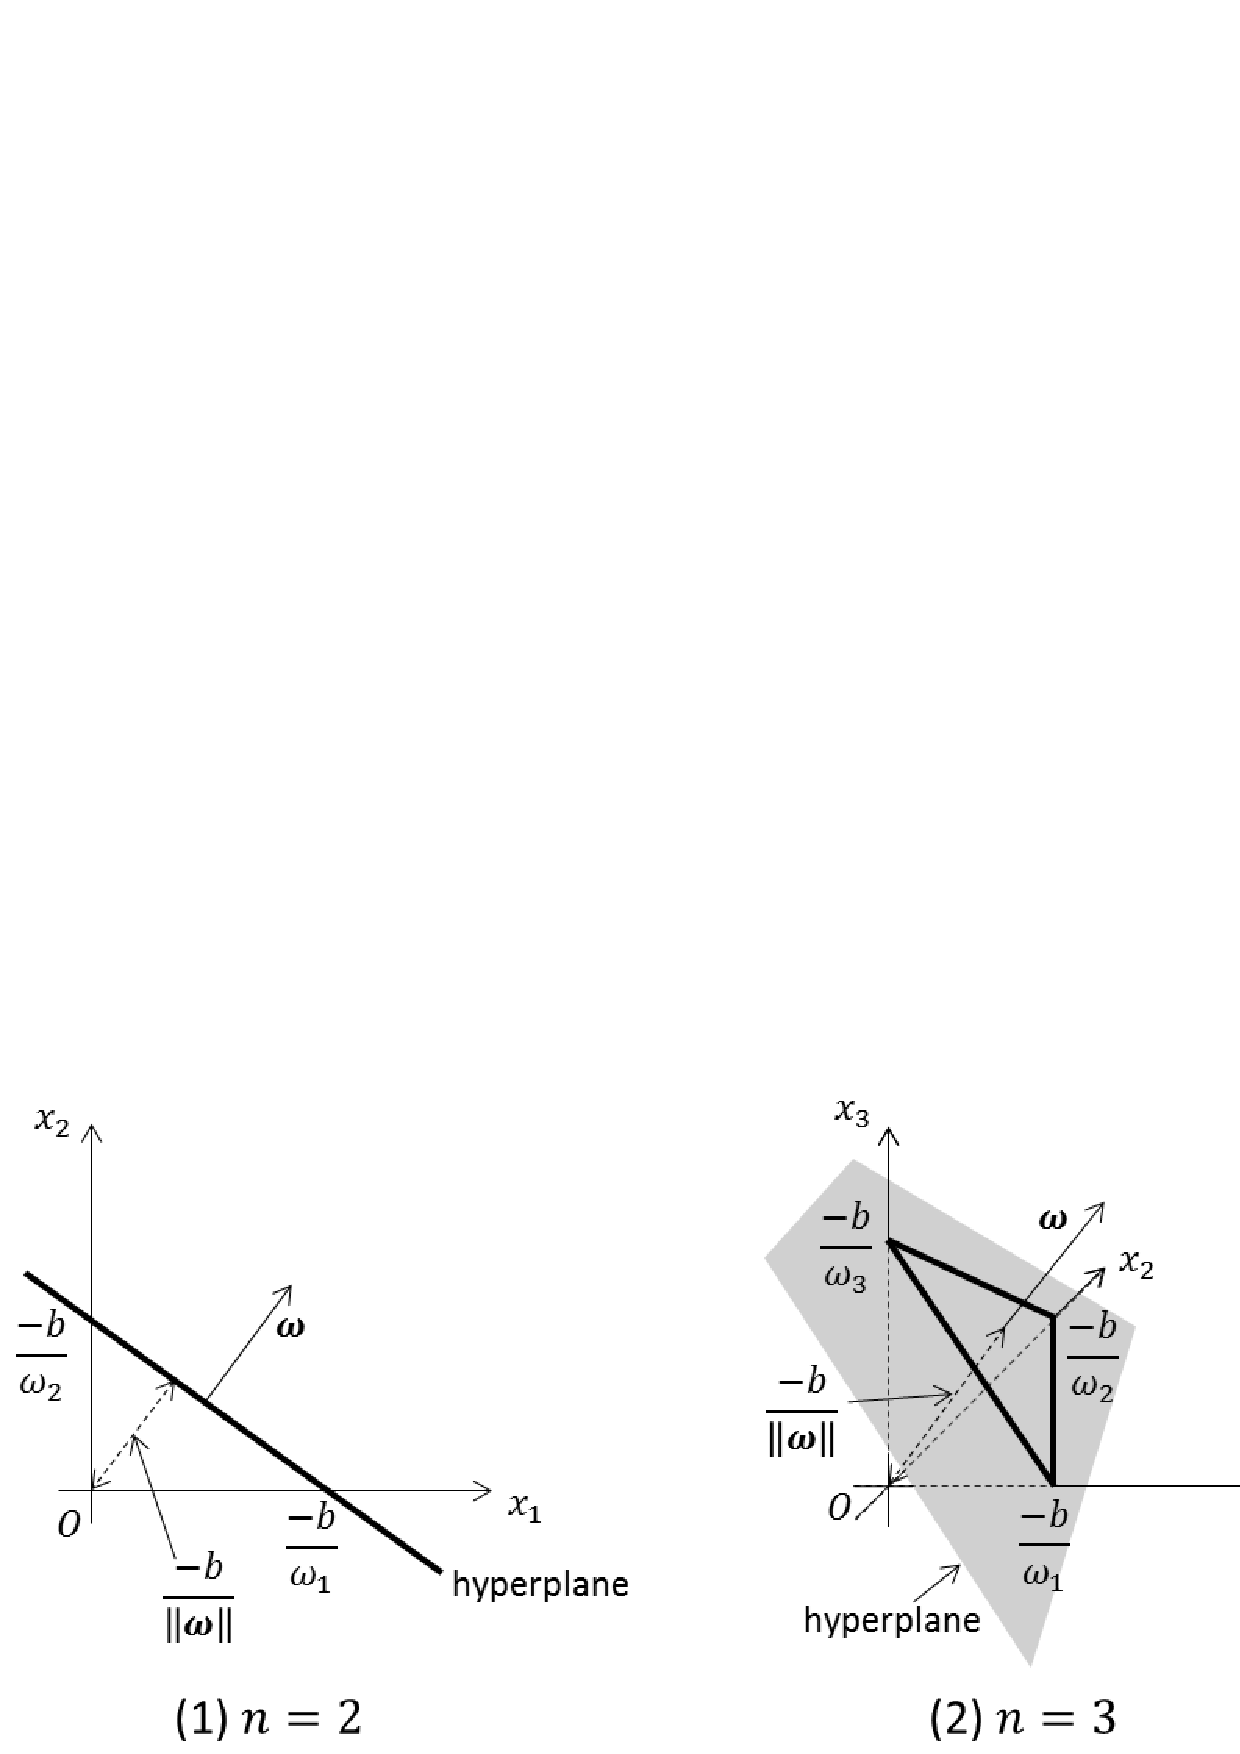
\includegraphics[width=110mm]{figure1.jpg}
\caption{The example of a learning process}
\label{fig:learning_process}
\end{figure}

\item 

(1) Will both classifiers converge?

Yes. For the linearly separable dataset, it is proved that the perceptron algorithm will converge, and the mistake bound is $R^2/\gamma^2$, which is independent from the order of the examples.

(2) What will be the training error of each one of the classifiers?

When both classifiers converge, no more mistakes will be made. In other words, the training error will be zero for both classifiers.

\item kernel function $K(x, y)$

$x$ and $y$ have the $same(x,y)$ values in common in their variables. Since we have at most $k$ variables in each conjunction, the number of all the combination of the same variables of size at most $k$ will be the kernel function. Thus,
\[
K(x, y)={}_{same(x,y)} C _1 + {}_{same(x,y)} C _2 + \cdots + {}_{same(x,y)} C _k
\]

\end{enumerate}

\section{Programming Assignment}
\begin{enumerate}
\item Feature Representation

\item Implementation


\item Experiments


\end{enumerate}


\end{document}

